\documentclass[12pt]{article}
 
%Russian-specific packages
%--------------------------------------
\usepackage[T2A]{fontenc}
\usepackage[utf8]{inputenc}
\usepackage[english, russian]{babel}
%for search in russian
\usepackage{cmap}
%--------------------------------------

%Math-specific packages
%--------------------------------------
\usepackage{amsmath}
\usepackage{amssymb}

%Format-specific packages
%--------------------------------------
\usepackage[left=2cm,
            right=2cm,
            top=2cm,
            bottom=2cm,
            bindingoffset=0cm]{geometry}
%--------------------------------------

% for theorems, lemmas and definitions
%--------------------------------------
\usepackage{amsthm}

\counterwithin*{equation}{section}

\newtheorem{definition}{Опр.}
\newtheorem{lemma}{Лемма}
\newtheorem*{remark}{Замечание}
\newtheorem*{corollary}{Следствие}
\newtheorem*{proposition}{Предложение}
\newtheorem*{example}{Пример}

\newtheoremstyle{basic_theorem}    %<name>
                 {\topsep}   %<space above>
                 {\topsep}   %<space below>
                 {\itshape}  %<body font>
                 {}          %<indent amount>
                 {\bfseries} %Theorem head font>
                 {.}         %<punctuation after theorem head>
                 {\newline}  %<space after theorem head> (default .5em)
                 {}          %<Theorem head spec>
\theoremstyle{basic_theorem}
\newtheorem{theorem}{Теорема}

\newtheoremstyle{name_theorem}
                {\topsep}
                {\topsep}
                {\itshape}
                {}
                {\bfseries}
                {}
                {\newline}
                {\thmnote{#3}}
\theoremstyle{name_theorem}
\newtheorem*{named_theorem}{Теорема}
%--------------------------------------

% For images
%--------------------------------------
\usepackage{wrapfig}
\usepackage{graphicx}
\graphicspath{ {./images/} }

%--------------------------------------

% My commands
%--------------------------------------
% for definitions
\newcommand\defin[1]{\textbf{#1}}

\def\eps{
    \varepsilon
}
\def\Eps{
    \mathcal{E}
}

\def\R{
    \mathbb{R}
}

\def\E{
    \mathrm{E}
}

\def\D{
    \mathrm{D}
}

\def\P{
    \mathrm{P}
}

\def\littleO{
    \overline{\overline{o}}
}

%--------------------------------------

\begin{document}

\section{Асимптотические оптимальные оценки}
    Пусть сл. векторы $\xi_n, \xi \in \R^K$, и определены на $(\Omega, \mathcal{F}, \P)$.
Пусть функция распределения $\xi_n$ есть $F_n(x)$, хар. ф-ция есть $\phi_n(t)$, а распределение
есть $Q_n$. Для вектора $\xi$ функцию распределения, хар. ф-цию и распреденеие обозначим $F(x)$,
$\phi(t),\ Q$ соответственно.

\begin{definition}
    Функция распределения $F_n(x)$ сходится к $F(x)$ при $n \rightarrow \infty$ в основном
    (пишем $F_n(x) \Rightarrow F$), если $F_n(x) \rightarrow F(x) \ \forall x \in C(F)$
\end{definition}

\begin{definition}
    Распределение $Q_n$ сходится к распределению $Q$ слабо (пишем $Q_n \xrightarrow{w} Q$),
    если $\forall$ непреревной и ограниченной $g: \R^K \rightarrow \R^1$
    $$ \int_{\R^K} g(x)Q_n(dx) \rightarrow \int_{\R^K} g(x)Q(dx)$$
    или, эквивалентно, $\E g(\xi_n) \rightarrow \E g(\xi)$.
\end{definition}

\begin{theorem}
    Следующие условия эквивалентны:
    \begin{enumerate}
        \item $F_n(x) \Rightarrow F$
        \item $Q_n \xrightarrow{w} Q$
        \item $\phi_n(t) \rightarrow \phi \ \forall t \in \R^K$
    \end{enumerate}
    Если выполненое любое из условий $1 - 3$, будем писать
    $\xi_n \xrightarrow{d} \xi$ и говорить, что $\xi_n$ сходится к $\xi$ по распределению.
\end{theorem}

\begin{theorem}[О наследовании сходимости]
\label{th::inherit_conv}
    Пусть сл. векторы $\xi_n, \xi \in \R^K, H: \R^K \rightarrow \R^1$ 
    Тогда:
    \begin{enumerate}
        \item Если $\xi_n \xrightarrow{d} \xi$, то $H(\xi_n) \xrightarrow{d} H(\xi)$
        \item Если $\xi_n \xrightarrow{\P} \xi$, то $H(\xi_n) \xrightarrow{\P} H(\xi)$
    \end{enumerate}
\end{theorem}

\begin{named_theorem}[Лемма Слуцкого]
\label{th::slut}
    Пусть $\xi_n, \xi, \eta_n, a \in \R^1, \xi_n \xrightarrow{d} \xi$, а $\eta_n \xrightarrow{\P} a$.
    Тогда:
    \begin{enumerate}
        \item \label{th::slut:sum} $\xi_n + \eta_n \xrightarrow{d} \xi + a$
        \item \label{th::slut:mult} $\xi_n \eta_n \xrightarrow{d} a\xi$
    \end{enumerate}
\end{named_theorem}
\begin{proof}
    Достаточно показать, что вектор
    \begin{equation} \label{eq::LemmaSlut}
        (\xi_n, \eta_n)^T \xrightarrow{d} (\xi, a)^T 
    \end{equation}
    Действительно, если \eqref{eq::LemmaSlut} верно, то при $H(x, y) = x + y$ в силу Теоремы \ref{th::inherit_conv} получаем пункт \ref{th::slut:sum} леммы,
    а при $H(x, y) = xy$ -  пункт \ref{th::slut:mult}.

    Для доказательства \ref{th::slut:sum}, проверим, что хар. ф-ция
    вектора $(\xi_n, \eta_n)^T$ сходится к хар. функции вектора $(\xi, \eta)^T$.
    Имеем: 
    $$|\E e^{it\xi_n + is\eta_n} - \E e^{it\xi + isa}| \leq | \E e^{it\xi_n + is\eta_n} - \E e^{it\xi_n + isa}| + | \E e^{it\xi_n + isa} - \E e^{it\xi + isa}| = \alpha_n + \beta_n$$

    $$\alpha_n \leq \E |e^{it\xi_n}(e^{it\eta_n + isa})| = \E |e^{it\eta_n + isa}| = \E g(\eta_n), \ g(x):= |e^{isx} - e^{isa}|$$
    Ф-ция g(x) непрерывна и ограничена, а т.к. $\eta_n \xrightarrow{d} a$,
    то в силу Теоремы \ref{th::inherit_conv} $\E g(\eta_n) \rightarrow \E g(a) = 0$
    Итак, $\alpha \rightarrow 0$.

    $$\beta_n = |\E e^{isa}(e^{it\xi_n} - e^{it\xi})| = |e^{isa} \E (e^{it\xi_n} - e^{it\xi})| = |\E (e^{it\xi_n} - e^{it\xi})| \rightarrow 0$$
    т.к. $\xi_n \xrightarrow{d} \xi$ и $\phi_n(t) \rightarrow \phi(t)$.
\end{proof}

Пусть наблюедние $X \sim  P_{\theta},\ \theta \in \Theta \subseteq \R^{K}$, а $\hat{\theta}_n$ - оценка $\theta$

\begin{definition}
    Если $n^{1/2}(\hat{\theta}_n - \theta) \xrightarrow{d} N(0, \Sigma(\theta)) \ \forall \theta \in \Theta$
    и ковариционная матрица $0 < \Sigma(\theta) < \infty$, то $\hat{\theta}_n$ называется асимптотической нормальной оценкой.
\end{definition}

\begin{definition}
    Если $\hat{\theta}_n \xrightarrow{\P} \theta \ \forall \theta \in \Theta$, то $\hat{\theta}_n$ называется состоятельной оценкой.
\end{definition}

\begin{remark}
    Дальше $\theta \in \Theta \subseteq \R^1$, то есть $\theta$ и $\hat{\theta}_n$ - скаляры.
\end{remark}

Если $\hat{\theta}_n$ - состоятельная оценка $\theta$, то при больших и $\hat{\theta}_n \approx \theta$ с вероятностью, близкой к единице.  

Если $\hat{\theta}_n$ - асимптотическая нормальная оценка $\theta$ (так как $\theta$ и $\hat{\theta}_n$ скаляры:

$n^{1/2}(\hat{\theta}_n - \theta) \xrightarrow{d} N(0, \sigma^2(\theta)) \ 0 < \sigma^2 < \infty,\ \forall \theta \in \Theta$), то: \begin{enumerate}

    \item $\hat{\theta}_n$ - состоятельная оценка $\theta$, так как $\hat{\theta}_n - \theta = n^{-1/2} n^{1/2}(\hat{\theta}_n - \theta) \xrightarrow{\P} 0$ 
        в силу п. \ref{th::slut:mult} леммы Слуцкого.
    \item Скорость сходимости $\hat{\theta}_n$ к $\theta$ есть $O(n^{1/2})$
    \item При больших $n$ со сл. в. $n^{1/2}(\hat{\theta}_n - \theta)$ можно обращаться (с осторожностью!) как с Гауссовской величиной. 
        
    Например, пусть дисперсия предельного Гауссовского закона $\sigma^2(\theta)$ будет непреревной ф-цией $\theta$. Тогда
        $$ \frac{n^{1/2}(\hat{\theta}_n - \theta)}{\sigma(\hat{\theta}_n)} =
        \underbrace{\frac{n^{1/2}(\hat{\theta}_n - \theta)}{\sigma(\theta)}}_{\xrightarrow{d} N(0, 1)}
        \underbrace{\frac{\sigma(\theta)}{\sigma(\hat{\theta}_n)}}_{\xrightarrow{\P} 1} \xrightarrow{d} \eta \sim N(0, 1)$$
        в силу п. 2 леммы Слуцкого. Значит,
        $$\P_\theta (|\frac{n^{1/2}(\hat{\theta}_n - \theta)}{\sigma(\hat{\theta}_n)}| < \xi_{1 - \alpha/2}) \rightarrow \P(|\eta| < \xi_{1 - \alpha/2}) = 1 - \alpha$$

        То есть примерно с вероятностью $1 - \alpha$ выполнено неравенство, или эквивалентно раскроем по модулю
        $$\underbrace{\hat{\theta}_n - n^{-1/2}\sigma(\hat{\theta}_n)\xi_{1 - \alpha /2} < \theta < \hat{\theta}_n + n^{-1/2}\sigma(\hat{\theta}_n)\xi_{1 - \alpha /2}}_{\mbox{Асимптотический доверительный интервал уровня $1 - \alpha$}}$$

    \item Асимптотические Гауссовские оценки можно сравнивать между собой: \\
    Если $n^{1/2} (\hat{\theta}_{i,n} - \theta) \xrightarrow{d} N(0, \sigma^2_{i}(\theta)),\ i = 1, 2, \ldots$, то
    можно посчитать асимптотическую относительную эффективность (АОЭ): 
    $$e_{1,2} = \frac{\sigma_2^2(\theta)}{\sigma_1^2(\theta)}$$
    Напомним, $e_{1, 2} = \lim_{n \to \infty} \frac{n'(x)}{n (x)}, \mbox{ где }
    n^{1/2}(\hat{\theta}_{1,n} - \theta) \xrightarrow{d} N(0, \sigma_1^2(\theta))$
    и $n^{1/2}(\hat{\theta}_{2,n'} - \theta) \xrightarrow{d} N(0, \sigma_1^2(\theta))$.
\end{enumerate}

    Вопрос: Есть ли такая оценка $\theta^*_n$, что АОЭ $e_{\theta^*_n, \hat{\theta}_n}(\theta) \geq 1 \ \forall \hat{\theta}_n$
    и всех $\theta \in \Theta$, то есть эффективнее всех остальных?
    
    Если да, то $\theta^*_n$ требует не больше наблюдений, чем любая $\hat{\theta}_n$, чтобы достичь одинаковой с $\hat{\theta}_n$ точности.
    Ясно, что пределеная дисперсия $n^{1/2}(\theta^*_n - \theta)$ должна быть не больше асимптотической дисперсии
    $n^{1/2}(\hat{\theta}_n - \theta)$ для любой асимптотической Гауссовской оценки $\hat{\theta}_n$. Но
    какова самая маленькая асимптотическая дисперсия у $n^{1/2}(\hat{\theta}_n - \theta)$?
    
    \begin{named_theorem}[Теорема Бахадура]
        \label{th::bahadur}
        Пусть $X_1, \ldots, X_n$ - н. о. р. сл. в., $X_1$ имеет
        плотность вероятности $f(x, \theta),\ \theta \in \Theta \subseteq \R^1$,
        по мере $\nu$. Пусть выполнены следующие условия:
        \begin{enumerate}
            \item $\Theta$ - интервал.
            \item Носитель $N_f = \{x: f(x, \theta) > 0\}$ не зависит от $\theta$.
            \item \label{th::bahadur:density} $\forall x \in N_f$ плотность $f(x, \theta)$ дважды непрерывно
                дифференцируема по $\theta$
            \item \label{th::bahadur:integral} Интеграл $\int f(x, \theta)\nu(dx)$  можно
                дважды дифференцировать по $\theta$, внося знак
                дифференцирования под знак интеграла.
            \item Информация Фишера $0 < i(\theta) < \infty \ \forall \theta \in \Theta$
            \item \label{th::bahadur:second_partial} $|\frac{\partial^2}{\partial \theta^2} \ln(f(x, \theta))| \leq M(x) \ \forall x \in N_f, \ \theta \in \Theta, \ \E_\theta M(X_1) < \infty$ 
        \end{enumerate}
        Тогда, если $n^{1/2}(\hat{\theta}_n - \theta) \xrightarrow{d} N(0, \sigma^2(\theta))$,
        то $\sigma^2(\theta) \geq \frac{1}{i(\theta)}$ всюду за исключением
        множества Лебеговой меры нуль.
    \end{named_theorem}
    \begin{remark}
        Если вдобавок $\sigma^2(\theta)$ и $i(\theta)$ непрерывны,
        то $\sigma^2(\theta) \geq \frac{1}{i(\theta)}$ при всех $\theta \in \Theta$.
    \end{remark}
    \begin{proof}
        Без доказательства.
    \end{proof}

    \begin{definition}
        Если $\theta, \hat{\theta}_n \in \R^1$ и $n^{1/2}(\hat{\theta}_n - \theta)\xrightarrow{d} N(0, \frac{1}{i(\theta)}),
        \ n \rightarrow \infty, \ \forall \theta \in \Theta,$
        причем $0 < i(\theta) < \infty$, то $\hat{\theta}_n$ называется \defin{асимптотически 
        эффективной оценкой}.
    \end{definition}
    Вопрос: Вообще можно ли найти такую оценку $\hat{\theta}_n$? Да
    
    \newpage
    
    Дальше $X = (X_1, \ldots, X_n), \ X \sim \P_\theta,\ \theta \in \Theta \subseteq \R^1$.
    \underline{Условие (A)}:
    \begin{enumerate}
        \item $\Theta$ - интервал, $\P_{\theta_1} \neq P_{\theta_2}$ при $\theta_1 \neq \theta_2$.
        \item $X_1, \ldots, X_n$ - независимые одинаково распределенные случайные величины
        \item $X_1$ имеет плотность вероятности $f(x, \theta)$ по мере $\nu$
        \item Носитель $N_f = \{x: f(x, \theta) > 0\}$ не зависит от $\theta$.
        \item Плотность вектора $X$ есть $p(x, \theta) = \prod_{i=1}^n f(x_i, \theta)$.
    \end{enumerate}
    \begin{definition}
    Функция $p(X, \theta)$ как функция $\theta$ при фиксированном $X$ называется
    \defin{правдоподобием} функции.
    $$L_n(X, \theta) = \ln p(X, \theta) = \sum_{i=1}^n \ln f(X_i, \theta)$$ 
    называется логарифмическим правдоподобием.
    \end{definition}

    Пусть $\theta_0$ будет истинное значение параметра.
    \begin{lemma}[Неравенство Йенсена]
        Пусть $g(x)$ выпукла книзу борелевская функция, $\E|\xi| <\infty$,
        $\E|g(\xi)| <\infty$. Тогда $g(\E\xi) \leq \E g(\xi)$. Если $\xi$
        не является почти наверное константой и $g$ строго выпукла, то неравенство строгое.
    \end{lemma}
    \begin{theorem}[Экстремальное свойство правдоподобия]
        \label{th::extr_plausibility}
        Пусть выполнено Условие (A). Пусть $E_{\theta_0} |\ln f(X_1, \theta)| < \infty,\ \forall \theta \in \Theta$.
        Тогда 
        $$\P_{\theta_0}(p(X, \theta_0) > p(X, \theta)) \rightarrow 1,\ n\rightarrow \infty,\ \theta_0 \neq \theta$$
    \end{theorem}
    \begin{proof}
        $$p(X, \theta_0) > p(X, \theta) \Leftrightarrow \ln p(X, \theta_0) > \ln p(X, \theta) \Leftrightarrow$$
        $$\eta_n := n^{-1} \sum_{i=1}^n \ln \left(\frac{f(X_i, \theta)}{f(X_i, \theta_0)}\right) < 0$$
    То есть надо показать, что $\P_{\theta_0}(\eta_n < 0) \rightarrow 1$. Но по слабому закону больших чисел:
    $$\eta_n = n^{-1}\sum \ln \left(\frac{f(X_i, \theta)}{f(X_i, \theta_0)} \right) \xrightarrow{\P}
    E_{\theta_0}\ln \left(\frac{f(X_1, \theta)}{f(X_1, \theta_0)} \right) $$

    Возьмем функцию $-\ln x$ - строго выпукла вниз и $\frac{f(X_1, \theta)}{f(X_1, \theta_0)}$
    не является п.н. константой (так как иначе если плотности п.н. совпадают,
    то и распределения при разных значениях совпадают, что противоречит Условию(A)(1)). 

    В силу неравенства Йенсена:
    $$\E_{\theta_0} \ln \frac{f(X_1, \theta)}{f(X_1, \theta_0)} < \ln \E_{\theta_0} \frac{f(X_1, \theta)}{f(X_1, \theta_0)} = \ln \int_{N_f} \frac{f(x, \theta)}{f(x, \theta_0)} f(x, \theta_0) \nu(dx) = \ln1 = 0$$
    Но если $\eta_n$ сходится по вероятности к отрицательному числу, то $P_{\theta_0}(\eta_n < 0) \rightarrow 1$
\end{proof}
    В силу теоремы \ref{th::extr_plausibility} естественно брать
    оценкой то значение $\theta$, которое максимизирует $p(X, \theta)$ при данном $X$

    \begin{definition}
        Случайная величина $\hat{\theta}_n \in \Theta$ называется
        \defin{оценкой максимального правдоподобия (о.м.п.)}, если
        $p(X, \hat{\theta}_n) = \max_{\theta\in\Theta} p(X, \theta)$,
        или эквивалентно $L_n(X, \hat{\theta}_n) = max_{\theta\in\Theta} L_n(X, \theta)$
    \end{definition}
    Итак, о.м.п $\hat{\theta}_n = \arg\max_{\theta\in\Theta} L_n(X, \theta)$.
    
    Если в $\forall\theta\in\Theta$ максимум не достигается, то о.м.п. не существует.

    Если $\Theta$ - интервал, $L_n(X, \theta)$ - гладкая по $\theta$ функция,
    то $\theta$ удовлетворяет уравнению правдоподобия
    \begin{equation} \label{eq::plausibility}
        \frac{\partial}{\partial\theta}L_n(X, \theta) = 0
    \end{equation}
    \begin{theorem}[О состоятельности решения уравнения правдоподобия]
        \label{th::consist_plausibility}
        Пусть выполнено Условие (А). Пусть $\forall x \in N_f \ \exists$ непрерывная
        производная $f'_{\theta}(x, \theta)$. Тогда уравнение \eqref{eq::plausibility}
        с вероятностью, стремящейся к 1 при $n\rightarrow \infty$ имеет решение $\in\Theta$.
        При этом среди всех такиъ решений есть такой корень $\hat{\theta}_n$, что он
        является состоятельнаой оценкой $\theta_0$
    \end{theorem}

    \begin{proof}
        Пусть $S_n = \{\omega\}$, при которых уравнение \eqref{eq::plausibility} имеет
        решение для $\theta\in\Theta$. Тогда теорема \ref{th::consist_plausibility} утверждает:
        \begin{enumerate}
            \item $P_{\theta_0}(S_n) \rightarrow 1$.
            \item Существует такое решение $\hat{\theta}_n \in \Theta$, что
                $$P_{\theta_0} (|\hat{\theta}_n - \theta_0| < \eps, S_n) \rightarrow 1,\ n\rightarrow\infty,\ \forall\eps>0$$
        \end{enumerate}
        \underline{Докажем пункт 1}: Выберем малое $a>0$ так, что на $(\theta_0 - a, \theta_0 + a) \subseteq\Theta$. Пусть
        $$S^a_n = \{\omega: L_n(X, \theta_0) > L_n(X, \theta_0 - a), L_n(X, \theta_0) > L_n(X, \theta_0 + a)\}$$
        В силу теоремы \ref{th::extr_plausibility} $\P_{\theta_0}(S_n^a) \rightarrow 1$

        При $\omega\in S_n^a$ функция $L_n(X, \theta)$ имеет
        локальный максимум $\hat{\theta}^a_n$ на интервале $(\theta_0 - a, \theta_0 + a)$
        \begin{figure}[h]
            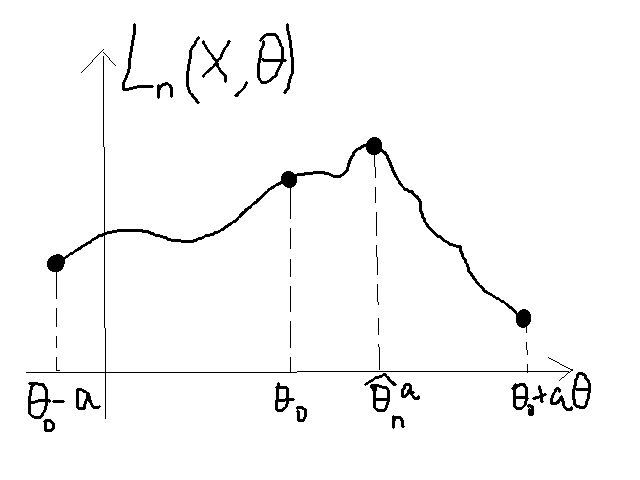
\includegraphics[width=0.4\textwidth]{L_n_func}
        \end{figure}
        
        Значит, $\frac{\partial}{\partial\theta}L_n(X, \hat{\theta}_n^a) = 0$.
        Тогда $\P_{\theta_0}(S_n) \geq \P_{\theta_0}(S_n^a) \rightarrow 1$, так
        как $S_n^a \subseteq S_n$, и пункт 1 доказан.

        \underline{Докажем пункт 2}: $\forall n$ при $\omega\in S_n$ может сущестовать целое множество корней
        $\{\theta^*_n\}$. Выберем в этом множестве корень $\hat{\theta}_n$,
        ближайший к $\theta_0$. Это можно сделать, так как
        функция $\frac{\partial}{\partial\theta} L_n(x, \theta)$ непрерывна по $\theta$,
        и последовательность корней есть корень. Этот корень $\hat{\theta}_n$
        и есть состоятельная оценка $\theta$. Покажем это:

        $\forall \text{ малого } \eps > 0$:
        \begin{equation}
            \label{eq::S_n}
            \P_{\theta_0}(|\hat{\theta}_n - \theta_0| < \eps, S_n) \geq
            \P_{\theta_0}(|\hat{\theta}^\eps_n - \theta_0| < \eps, S_n^\eps)
        \end{equation}
        Так как $S^\eps_n \subseteq S_n,\
        (\omega: |\hat{\theta}^\eps_n - \theta_0| < \eps) \subseteq
        (\omega: |\hat{\theta}_n - \theta_0| < \eps)$
        
        Но $\P_{\theta_0}(|\hat{\theta}^\eps_n - \theta_0| < \eps, S^\eps_n) 
        \underset{\text{т.к. события из } S_n^\eps \text{ лежат в } |\hat{\theta}^\eps_n - \theta_0| < \eps}{=}
        \P_{\theta_0}(S_n^\eps) \rightarrow 1$, значит в силу \eqref{eq::S_n}
        $$\P_{\theta_0} (|\hat{\theta}_n - \theta_0| < \eps, S_n) \rightarrow 1$$
    \end{proof}

    \begin{remark}
        Пусть 
        $$\theta^*_n = \begin{cases}
            \text{сост. корню уравнения правдоподобия, если он сущ.} \\
            \theta',\ \theta'\in\Theta, \text{иначе}
        \end{cases}$$
        Тогда случайная величина $\theta^*_n$ всегда определена, и
        $\theta^*_n \xrightarrow{\P} \theta_0$, так как
        $$\P(|\theta^*_n - \theta_0| < \eps) =
        \P(|\hat{\theta}_n - \theta_0| < \eps, S_n) +
        \P(|\theta' - \theta_0| < \eps, \overline{S}_n) \rightarrow 1$$
        Ясно, что 
        \begin{equation}
            \frac{\partial}{\partial\theta} L_n(X, \theta^*_n) = \littleO_p(1)
        \end{equation}
        Так как производная отлична от нуля только на $\overline{S}_n$.

        Будем называть $\theta_n^*$ \defin{обобщенным состоятельным корнем уравнения
        правдоподобия}
    \end{remark}

    \begin{theorem}[Об асимптотической эффективности состоятельности решения]
        \label{th::asympt_consist}
        Пусть $X = (X_1, \ldots, X_n),\ \{X_i\}$ - н.о.р. сл.в., и
        удовлетворяются предположения Теоремы Бахадура, в которых условия
        \ref{th::bahadur:density} и \ref{th::bahadur:second_partial} заменены на
        предположения о третьей, а не второй производной. То есть
        $$|\frac{\partial^3}{\partial \theta^3} \ln f(x, \theta)| \leq M(x) \ \forall x\in N_f,\ \forall\theta\in\Theta,\ \E_{\theta_0}M(X_1) < \infty$$
        Тогда, если $\theta^*_n$ - обобщенный состоятельный корень из теоремы \ref{th::consist_plausibility}, то
        $$\sqrt{n}(\theta^*_n - \theta_0) \xrightarrow{d} N(0, \frac{1}{i(\theta_0)})$$
        То есть $\theta^*_n$ - асимптотическая эффективная оценка.
    \end{theorem}
    \begin{proof}
        Будем обозначать $\frac{\partial}{\partial\theta}L_n(X, \theta), \frac{\partial^2}{\partial\theta^2}L_n(X, \theta), \ldots$
        через $L'_n(\theta), L^{(2)}_n(\theta), \ldots$.

        Для фиксированного $X$ в силу формулы Тейлора и последнего замечания:
        $$\littleO_p(1) = L'_n(\theta^*_n) = L'_n(\theta_0) + L^{(2)}_n(\theta_0)(\theta^*_n - \theta_0) + 
        \frac{1}{2}L_n^{(3)}(\widetilde{\theta}_n)(\theta^*_n - \theta_0)^2,\ \widetilde{\theta}_n \in(\theta_0, \theta_n^*)$$
        Отсюда,
        \begin{equation}
            \label{eq::taylor_frac}
            n^{1/2}(\theta^*_n - \theta_0) = -\frac{n^{-1/2} L'_n(\theta_0) + \littleO_p(1)}{n^{-1}(L^{(2)}_n(\theta_0) + \frac{1}{2}L^{(3)}_n(\widetilde{\theta}_n)(\theta^*_n - \theta_0))}
        \end{equation}
        \underline{Рассмотрим числитель \eqref{eq::taylor_frac}} и покажем, что
        \begin{equation}
            \label{eq::taylor_frac::num}
            n^{-1/2}L_n'(\theta_0) = n^{-1/2}\sum_{i=1}^n \frac{f'_\theta(X_i, \theta_0)}{f(X_i, \theta_0)} \xrightarrow{d} \xi\sim N(0, i(\theta_0))
        \end{equation}
        Действительно, 
        $$\E_{\theta_0}\frac{f'_{\theta_0}(X_1, \theta_0)}{f(X_i, \theta_0)} = \int_{N_f}\frac{f'_\theta(x, \theta_0)}{f(x,\theta_0)} f(x,\theta_0) \nu(dx) = 0$$
        $$\D_{\theta_0}\frac{f'_{\theta_0}(X_1, \theta_0)}{f(X_i, \theta_0)} = \E_{\theta_0}\left(\frac{\partial}{\partial\theta}\ln f(X_1, \theta_0)\right)^2 - \underbrace{\left(\E_{\theta_0}\frac{f'_{\theta_0}(X_1, \theta_0)}{f(X_i, \theta_0)}\right)^2 }_{ =\ 0} \underset{\text{по опр.}}{=} i(\theta_0)$$
        Так как $f, f'$ - борелевские функции, то случайные величины $\{\frac{f'_\theta(X_i, \theta_0)}{f(X_i, \theta_0)},\ i=1,\ldots,n\}$ - н.о.р.,
        соотношение \eqref{eq::taylor_frac::num} следует из Центр. пред. Теоремы.
        
        В силу Леммы Слуцкого числитель \eqref{eq::taylor_frac} $\xrightarrow{\P} N(0, i(\theta_0))$

        Теперь \underline{рассмотрим знаменатель \eqref{eq::taylor_frac}}:
        \begin{equation}
            \label{eq::taylor_frac::den}
            n^{-1}L_n^{(2)}(\theta_0) = n^{-1}\sum^n_{i=1}\left[ \frac{f^{(2)}_\theta(X_i, \theta_0)}{f(X_i, \theta_0)} - \left(\frac{f'_\theta(X_i, \theta_0)}{f(X_i, \theta_0)}\right)^2\right] \xrightarrow{\P} -i(\theta)
        \end{equation}
        Действительно, в силу ЗБЧ
        $$n^{-1}\sum^n_{i=1} \frac{f^{(2)}_\theta(X_i, \theta_0)}{f(X_i, \theta_0)} \xrightarrow{\P} \E_{\theta_0}\frac{f^{(2)}_\theta(X_1, \theta_0)}{f(X_1, \theta_0)} = \int_{N_f} \frac{f^{(2)}_\theta(x, \theta_0)}{f(x, \theta_0)} f(x, \theta_0) \nu(dx) = 0$$
        $$n^{-1}\sum^n_{i=1} \left(\frac{f'_\theta(X_i, \theta_0)}{f(X_i, \theta_0)}\right)^2 \xrightarrow{\P} E_{\theta_0} \left(\frac{\partial}{\partial\theta} \ln f(X_1, \theta_0)\right)^2 = i(\theta)$$
    
    Применяя лемму Слуцкого, получим \eqref{eq::taylor_frac::den}.

    Далее рассмотрим второе слагаeмое в знаменете \eqref{eq::taylor_frac}
    \begin{equation}
        \label{eq::taylor_frac::den2}
        |\frac{1}{2n} L_n^{(3)}(\widetilde{\theta}_n)(\theta^*_n - \theta_0)| \leq \frac{1}{2}|\theta_n^* - \theta_0| n^{-1} \sum_{i=1}^n M(X_i) \xrightarrow[\text{л. Слуцкого}]{\P} 0
    \end{equation}
    
    В силу \eqref{eq::taylor_frac::den} и \eqref{eq::taylor_frac::den2} и Леммы Слуцкого
    знаменатель \eqref{eq::taylor_frac} сходится по вероятности к $-i(\theta_0)$

    Значит, что вся дробь \eqref{eq::taylor_frac} сходится по распределению к
    $\frac{1}{i(\theta_0)} \xi \sim N(0, \frac{1}{i(\theta_0)})$
\end{proof}

\subsection*{Оценки максимального правдоподобия для векторого параметра}
    Пусть $X = (X_1, \ldots, X_n)$ - н.о.р., $X_1 \sim f(x, \theta),\ \theta\in\Theta\subseteq\R^k,\
    \Theta$ - открытое множество

    Тогда логарифмические правдоподобие имеет вид 
    $$L_n(X, \theta) = \sum_{i=1}^n\ln f(X_i, \theta)$$
    
    Система уравнений правдоподобия
    \begin{equation*}
        \label{eq::sys_plausibility}
        \frac{\partial L_n(X, \theta)}{\partial\theta_i} = 0,\ i =1,2,\ldots,k
    \end{equation*}
    
    При условиях регулярности, похожих на условия теоремы \ref{th::asympt_consist},
    показыватся:
    \begin{enumerate}
        \item С вероятностью, стремящейся к единице при $n \rightarrow \infty$,
            система уравнений \eqref{eq::sys_plausibility} имеет такое решение $\hat{\theta}_n\in\Theta$,
            что $\hat{\theta}_n$ сходится к истинному значению $\theta_0$.
        \item Соответствующая оценка $\theta^*_n$ асимптотически нормальна. А именно
         $$n^{1/2}(\theta^*_n - \theta_0) \xrightarrow{d} N(0, I^{-1}(\theta_0)),\ n\rightarrow\infty$$
         Здесь $I(\theta) > 0$ - матрица информации Фишера, то есть
         $$I(\theta) = (I_{ij}(\theta)),\ I_{ij}(\theta) = \E_\theta \left\{\frac{\partial \ln f(X, \theta)}{\partial\theta_i} \cdot \frac{\partial\ln f(X, \theta)}{\partial\theta_j}\right\}$$ 
    \end{enumerate}
\begin{example}
        $X = (X_1, \ldots, X_n)$, где $\{X_i\}$ - н.о.р., $X_1 \sim N(0, \sigma^2),\ a < \theta < b$,
        $a$ и $b$ - известные конечные числа, дисперсия $\sigma^2$ известна.
        Построим асимптотически эффективную оценку $\theta^*_n$ для $\theta$.

        Здесь $p(x, \theta) = \left(\frac{1}{\sqrt{2\pi} \sigma}\right)^ne^{-\frac{1}{2\sigma^2}\sum_{i=1}^n (x_i-\theta)^2}$,
        значит
        $$L_n(X, \theta) = \ln\left(\frac{1}{\sqrt{2\pi}\sigma}\right)^n - \frac{1}{2\sigma^2}\sum_{i=1}^n(X_i-\theta)^2$$
        Уравнение правдоподобия имеет вид
        $$\frac{\partial L_n(X, \theta)}{\partial\theta} = \frac{1}{\sigma^2}\sum_{i=1}^n(X_i - \theta) = 0$$
        Его решение существует и единственно, это $\overline{X}$, причем
        в т. $\theta = \overline{X}\ L_n(X,\theta)$ достигает максимума,
        так как $\frac{\partial^2 L_n(X, \overline{X})}{\partial\theta^2} = - \frac{1}{\sigma^2} < 0$

        Таким образом, если $a < \overline{X} < b$, то о.м.п. сущесвтует и равна $\overline{X}$,
        в противном случае о.м.п. не существует. Если положить
        \begin{equation}
            \label{eq::ex::as_appraisal}
            \theta^*_n = \begin{cases}
                \overline{X},\ a < \overline{X} < b \\
                \frac{a+b}{2},\ \overline{X} \notin (a,b) 
            \end{cases}
        \end{equation}
        То в силу теоремы \ref{th::asympt_consist} (её условия
        выполнены, проверьте сами), $\theta^*_n$ - асимптотически эффективная оценка, то есть
        \begin{equation}
            \label{eq::ex::as_conv}
            n^{1/2}(\theta^*_n - \theta_0) \xrightarrow{d} N(0, \sigma^2)
        \end{equation}
        Напомним, что в этой модели $i(\theta) = \frac{1}{\sigma^2}$.
        Cправедливость \eqref{eq::ex::as_conv} c $\theta^*_n$
        из \eqref{eq::ex::as_appraisal} легко проверить непосредственно.
\end{example}
\begin{example}
    Если $\Theta$ - компакт (то есть отрезок $[a, b]$), то о.м.п. существует
    всегда, так как непрерывная функция на отрезке всегда достигает своего максимума.
    Значит значение о.м.п.
    \begin{equation*}
        \theta^*_n = \begin{cases}
            \overline{X},\ a < \overline{X} < b \\
            a,\ \overline{X} < a \\
            b,\ \overline{X} > b
        \end{cases}
    \end{equation*}
    Но на границах теряется асимптотическая Гауссовость.
\end{example}


\section{Проверка статистических гипотез}
$X = (X_1, \ldots, X_n)$ имеет плотность вероятности $p(X, \theta)$
по мере $\mu,\ \theta\in\Theta\subseteq\R^1$

\begin{definition}
    Предположение вида $H_0: \theta\in\Theta_0$, где
    $\Theta_0\in\Theta$, называется параметрической гипотезой.
    Альтернатива $H_1:\theta\in\Theta_1$, где
    $\Theta_1\in\Theta\backslash\Theta_0$
\end{definition}

\begin{definition}
    Если $\Theta_0(\Theta_1)$ состоит из одной точки,
    то гипотеза $H_0$ (альтернатива $H_1$) называется
    простой.
    В противном случае $H_0(H_1)$ - сложная
\end{definition}

\underline{Постановка задачи}:

Необходимо построить правило (статистический критерий - $test$),
который позволяет заключить, согласуется ли наблюдение $X$
с $H_0$ или нет.

\underline{Правило.}

Выберем в множестве значений $x$ вектора $X$ (у нас либо
$x = \R^n$, либо $x = N_p \subseteq \R^n$ - носитель
плотности) подмножество $S$. Если $X \in S$, то $H_0$ отвергается и
принимается $H_1$. Если $X \in \overline{S} = X \backslash S$, то
$H_0$ принимается.

\begin{definition}
    Множество $S$ называется критическим множеством или критерием,
    $\overline{S}$ - область принятия гипотезы.
\end{definition}

\begin{definition}  
    \defin{Ошибка 1-го рода} - принять $H_1$, когда
    верна $H_0$. Вероятность ошибки 1-го рода $\alpha
    = \P(H_1 | H_0)$ (это условная запись, а не условная вероятность). 
    \defin{Ошибка 2-го рода} - принять $H_0$, когда
    верна $H_1$. Вероятность ошибки 2-го рода $\beta
    = \P(H_0 | H_1)$.
\end{definition}

\begin{definition}
    \defin{Мощность критерия $S$} называется функция $W(S, \theta) = W(\theta)
    := \P_\theta(X\in S)$ (вероятность отвергнуть $H_0$, когда
    значение параметра есть $\theta$).
\end{definition}

Тогда
\begin{align*}
    \alpha &= \alpha(\theta) = W(\theta),\ \theta\in\Theta_0; \\
    \beta  &= \beta(\theta) = 1 - W(\theta),\ \theta\in\Theta_1
\end{align*}

\begin{definition}
Обычно $H_0$ более важна. Поэтому рассматривают критерии
такие, что 
$$\alpha(\theta) = W(\theta) = \P_{\theta}(X\in S) \leq\alpha \ \forall \theta\in\Theta_0$$
    Число $\alpha$ называют \defin{уровнем значимости критерия}.
    Пишут $S_\alpha$ - критерий уровня $\alpha$. Обычно $\alpha$ -
    маленькое число, которое мы задаем сами.
\end{definition}

\begin{definition}
    Если критерий $S^*_\alpha \in \{S_\alpha\}$ и $\forall\theta\in\Theta_1$ и
    $\forall S_\alpha \ W(S^*_\alpha,\theta) \geq W(S_\alpha, \theta)$,
    то критерий $S^*_\alpha$ называется \defin{РНМ-критерием (равномерно наиболее мощным)}.
\end{definition}

Если $H_0:\theta = \theta_0,\ H_1:\theta = \theta_1$ (то есть
$H_0$ и $H_1$ - простые), то задача отыскания РНМ-критерия
заданного уровня $\alpha$ имеет вид:
\begin{align*}
  \P_{\theta_0}(X\in S^*_\alpha) &\leq \alpha, \\
  \P_{\theta_1}(X\in S^*_\alpha) &\geq \P_{\theta_1}(X\in S_\alpha) \ \forall S_\alpha
\end{align*}

Положим для краткости:
$p_0(x) := p(x, \theta_0),\ \E_0 = \E_{\theta_0},\ p_{1}(x) = p(x, \theta_1),\ \E_1 = \E_{\theta_1}$

Введем множество
$$S(\lambda) = \{x: p_1(x) - \lambda p_0(x) > 0\}, \lambda > 0$$

\begin{theorem}[Лемма Неймана-Пирсона]
    \label{th::lemma_N_P}
    Пусть для некоторого $\lambda > 0$ и критерия $R$
    (когда $X$ попадает в $R$, то $H_0$ отвергается)
    выполнено:
    \begin{enumerate}
        \item  $\P_0(X\in R) \leq \P_0(X\in S(\lambda))$

        Тогда: 
        \item  $P_1(X\in R) \leq \P_1(X\in S(\lambda))$
        \item  $P_1(X\in S(\lambda)) \geq \P_0(X\in S(\lambda))$
    \end{enumerate}
\end{theorem}
\begin{remark}
    $X\in S(\lambda) \Leftrightarrow \frac{p_1(x)}{p_0(x)} > \lambda$.
    Так как $p_1(X)$ и $p_0(X)$ - правдоподобие, то критерий
    называется критерием отношения правдоподобия Неймана-Пирсона.
\end{remark}
\begin{remark}
    Утверждение 3 для $S(\lambda)$
    означает, что
    $$\P(H_1 | H_1) \geq \P(H_1|H_0) \Leftrightarrow W(S(\lambda), \theta_1) \geq W(S(\lambda), \theta_0)$$
    Это свойство назыается несмещенностью критерия $S(\lambda)$
\end{remark}
\begin{proof}
    Дальше для краткости $S(\lambda) = S$. Пусть
    $I_R(x) = \begin{cases}
        1, x\in \R \\
        0, x\notin \R 
    \end{cases}$, $I_S(x)$ определяем аналогично.
    Тогда Условие (А) имеет вид:
    \begin{equation}
        \label{eq::cond_A}
        \E_0I_R(x) \leq \E_0I_S(x)
    \end{equation}

    \underline{Докажем пункт 2}:
    Верно неравенство
    \begin{equation} \label{eq::LemmaNP::dens}
        I_R(x)[p_1(x) - \lambda p_0(x)] \leq I_S(x)[p_1(x) - \lambda p_0(x)]
    \end{equation}

    Действительно, если $(p_1(x) - \lambda p_0(x)) > 0$,
    то $I_S(x) = 1$ и \eqref{eq::LemmaNP::dens} очевидно.

    Если же $p_1(x) - \lambda p_0(x) \leq 0$, то правая часть
    \eqref{eq::LemmaNP::dens} есть ноль, а левая $\leq$ нуля.

    Итак, \eqref{eq::LemmaNP::dens} верно: интегрируем это неравенство по $x\in\R^n$:
    $$\E_1I_R(X) - \lambda\E_0I_R(X) \leq \E_1I_S(X) - \lambda\E_0I_S(X)$$
    \begin{equation} \label{eq::LemmaNP::MO}
        \E_1I_S(X) - \E_1I_R(X) \geq \lambda\underbrace{[\E_0I_S(X) - \E_0I_R(X)]}_{\geq 0 \text{ по условию \eqref{eq::cond_A}}}
    \end{equation}
    В силу \eqref{eq::cond_A}, \eqref{eq::LemmaNP::MO} и условия $\lambda > 0$ получаем:
        $$E_1I_S(X) \geq E_1I_\R(X)$$

    \underline{Докажем пункт 3}: Пусть $\lambda \geq 1$.
    Из определения $S\ p_1(x) > p_0(x) \ \forall x\in S.$
    Отсюда
    $$\P_0(X\in S) = \int_{R^n} I_S(X)p_0(x)\mu(dx) \leq \int_{R^n} I_S(X)p_1(x)\mu(dx) = \P_1(X\in S)$$ 
    То есть $\P(H_1 | H_0) \leq \P(H_1 | H_1)$

    Пусть $\lambda < 1$. Рассмотрим $\overline{S} = \{x: p_1(x) \leq \lambda p_0(x)\}$.
    При $\lambda < 1\ p_1(x) < p_0(x)$ при $x\in \overline{S}$.
    Отсюда
    $$\P_1(X\in \overline{S}) = \int_{R^n} I_{\overline{S}}(X)p_1(x)\mu(dx) \leq \int_{R^n} I_{\overline{S}}(X)p_0(x)\mu(dx) = \P_0(X\in \overline{S})$$ 
    То есть $1 - \P_1(X\in S) \leq 1 - \P_0(X\in S)$, откуда
    $\P_1(X\in S) \geq \P_0 (X\in S)$
\end{proof}

\begin{example}
    $X = (X_1,\ldots, X_n), \{X_i\}$ - н.о.р., $X_1 \sim N(\theta, \sigma^2)$,
    дисперсия $\sigma^2$ известна. Построим наиболее мощный критерий
    для проверки $H_0: \theta = \theta_0$ против $H_1: \theta = \theta_1$
    (в случае $\theta_1 > \theta_0$). Уровень значимости возьмем $\alpha$.
    \begin{enumerate}
        \item Имеем 
        $$p_0 = \left(\frac{1}{\sqrt{2\pi}\sigma}\right)^n \exp{\left\{-\frac{1}{2\sigma^2} \sum^n_{i=1} (x_i -\theta_0)^2\right\}},\ 
        p_1 = \left(\frac{1}{\sqrt{2\pi}\sigma}\right)^n \exp{\left\{-\frac{1}{2\sigma^2} \sum^n_{i=1} (x_i -\theta_1)^2\right\}};$$
        $$S(\lambda) = \{x:p_1(x) - \lambda p_0(x) > 0\} \underset{\text{делим на }p_0}{\Leftrightarrow}
        \exp{\left\{\frac{1}{2\sigma^2}\sum_{i=1}^n\left[ (x_i-\theta_1)^2 -(x_i-\theta_0)^2 \right]\right\}} > \lambda\Leftrightarrow$$
        $$\Leftrightarrow \sum_{i=1}^n\left[(x_i - \theta_1)^2 - (x_i - \theta_0)^2\right] < \lambda_1 = -2\sigma^2\ln\lambda
        \underset{\text{арифметика}}{\Leftrightarrow} (\theta_0 - \theta_1)\sum_{i=1}^n x_i \leq\lambda_2 \Leftrightarrow$$
        $$\Leftrightarrow \sum_{i=1}^n x_i > \widetilde{\lambda},\ \widetilde{\lambda}(\lambda, n, \sigma^2, \theta_0, \theta_1)$$
        Итак,
        $$S(\lambda) = \left\{x: \sum_{i=1}^n x_i > \widetilde{\lambda}\right\} \text{ при некотором } \widetilde{\lambda}$$

        \item Определим $\widetilde{\lambda} = \widetilde{\lambda}_\alpha$ 
            из уравнения
            $$\alpha = \P_{\theta_0}(X \in S(\widetilde{\lambda}_\alpha)) = 
            \P_{\theta_0}\left(\sum_{i=1}^n X_i > \widetilde{\lambda}_\alpha\right)$$
            Преобразуем левую сумму в стандартную Гауссовскую величину. Тогда
            $$\alpha = \P_{\theta_0}\left(\frac{1}{\sqrt{n} \sigma} \sum_{i=1}^n(X_i - \theta_0) > \frac{\widetilde{\lambda}_\alpha - n\theta_0}{\sqrt{n}\sigma}\right)=
            1 - \Phi\left(\frac{\widetilde{\lambda}_\alpha - n\theta_0}{\sqrt{\pi}\sigma}\right)$$
            так как $\frac{1}{\sqrt{n}\sigma}\sum_{i} (X_i - \theta_0) \sim N(0, 1)$ при $H_0$.
            
            Значит $\Phi\left(\frac{\widetilde{\lambda}_\alpha - n\theta_0}{\sqrt{\pi}\sigma}\right) = 1 - \alpha,\
            \left(\frac{\widetilde{\lambda}_\alpha - n\theta_0}{\sqrt{\pi}\sigma}\right) = \xi_{1-\alpha}$
             - квантиль станд. норм. закона уровня $1 - \alpha$.
            Окончательно, $\widetilde{\lambda}_\alpha = n\theta_0 + \sqrt{n}\sigma \xi_{1-\alpha}$

        \item Положим $S^*_{\alpha} = \{x: \sum_{i=1}^n x_i > \widetilde{\lambda}_\alpha\}$
            Тогда $\P_{\theta_0}(X\in S_\alpha^*)=\alpha,$ и: 
            $$\forall S_\alpha\ \P_{\theta_0}(X\in S_\alpha)\leq\alpha = \P_{\theta_0}(X\in S_\alpha^*)$$
        
            Значит, выполнено условие 1 Леммы Неймана-Пирсона, и в силу
            пункта 2 этой леммы
            $$\P_{\theta_1}(X\in S_\alpha) \leq \P_{\theta_1}(X\in S_\alpha^*)$$
            То есть $S_\alpha^*$ - наиболее мощный критерий уровня $\alpha$.
        \end{enumerate} 
        Так как $S^*_{\alpha}$ не зависит от $\theta_1$,
        то $S^*_{\alpha}$ - РНМ-критерий для $H_0: \theta = \theta_0$
        против $H^+_1 : \theta > \theta_1$
        Мощность критерия $S^*_{\alpha}$ для $H_0$ при альт. $H^+_1$

        $$W(\theta, S^*_{\alpha}) = \P_\theta\left(\sum_{i=1}^nX_i > n\theta_0 + \sqrt{n}\sigma\xi_{1-\alpha}\right) = $$
        $$ = \P_\theta\left(\frac{1}{\sqrt{n}\sigma} \sum_{i=1}^n(X_i - \theta) > \frac{\sqrt{n}(\theta_0 - \theta)}{\sigma} + \xi_{1-\alpha}\right) =
        1 - \Phi\left(\xi_{1-\alpha} + \frac{\sqrt{n}(\theta - \theta_0)}{\sigma}\right)$$
\end{example}

    \subsection*{О связи между доверительным оцениванием и проверкой гипотез}

\begin{definition}
    Случайное подмножесто $\Theta^*=\Theta*(X,\alpha)\subseteq\Theta$
    называется доверительным множеством уровня $1-\alpha,\ 0<\alpha<1$,
    если
    $$\P_\theta(\theta\in\Theta^*(X,\alpha))\geq 1-\alpha\ \forall\theta\in\Theta$$
\end{definition}
\begin{theorem} \label{th::trusted_set_eq_plausibility_test}
    \begin{enumerate}
    \item Пусть $\forall\theta_0\in\Theta$ гипотеза $H_0:\theta=\theta_0$
    при альтернативе $H_1:\theta\neq\theta_0$ имеет $S_\alpha(\theta_0)$
    критерием уровня $\alpha$. Пусть $\Theta^*(x,\alpha) = \{\theta:x\in\overline{S_\alpha}(\theta)\}$.
    тогда $\Theta^*(X,\alpha)$ - доверительное множество уровня $1-\alpha$.
    (Если есть критерий, то можно по этому  построить доверительное множество)
    
        \item Если $\Theta^*(X,\alpha)$ - доверительное множество уровня $1-\alpha$,
    то $\overline{S_\alpha}(\theta_0)=\{x:\theta_0\notin\Theta(x,\alpha)\}$
    есть обрасть применения гипотезы $H_0$ (следовательно и критерий).
    \end{enumerate}
\end{theorem}
\begin{remark}
    Пункт 2 означает, что если $\theta_0$ попало в доверительное множество,
    то $H_0$ надо применять.
\end{remark}
\begin{proof}
    \begin{enumerate}
        \item $$\P_\theta(\theta\in\Theta^*(X,\alpha)) = \P_\theta(X\in\overline{S_\alpha}(\theta)) = 1 - \underbrace{\P_\theta(X\in S_\alpha(\theta))}_{\leq\alpha}\geq 1-\alpha\ \forall\theta\in\Theta$$
        \item $$\P_{\theta_0}(X\in S_\alpha(\theta_0)) = 1-\P_{\theta_0}(X\in \overline{S_\alpha}(\theta_0))=
        1-\underbrace{\P_{\theta_0}(\theta_0\in\Theta^*(X,\alpha))}_{\geq 1-\alpha} \leq 1-(1-\alpha) = \alpha$$
    \end{enumerate}
\end{proof}
\begin{example}
    Пусть $X=(X_1,\ldots,X_n)$, $\{X_i\}$ - н.о.р. сл.в., $X_1\sim N(0,\sigma^2),\theta\in\R^1$.
    Построим критерий для $H_0:\theta=\theta_0$ против $H_1:\theta\neq\theta_0$.
    Уровень значимости пусть будет $\alpha,\ 0<\alpha<1$.
    
    Построим доверительное множество для $\theta$ уровня $1-\alpha$.
    Пусть $\overline{X}=\frac{1}{n}\sum^n_{i=1}X_i$ - оптимальная оценка $\theta$.
    Тогда $\frac{n^{1/2}(\overline{X}-\theta)}{\sigma}\sim N(0,1)$,
    $$\P_\theta\left(\lvert\frac{n^{1/2}(\overline{X}-\theta)}{\sigma}\rvert<\xi_{1-\alpha/2}\right) = 1-\alpha$$ 
    $$\Phi(\xi_{1-\alpha/2})=1-\alpha/2$$
    То есть $\Theta^*(X,\alpha)=\{\theta:\vert\frac{n^{1/2}(\overline{X}-\theta)}{\sigma}\vert<\xi_{1-\alpha/2}\}$.
    В силу замечания к Теореме \ref{th::trusted_set_eq_plausibility_test}
    $S_{\alpha}(\theta_0)=\{X:\vert\frac{n^{1/2}(\overline{X}-\theta_0)}{\sigma}\vert\geq\xi_{1-\alpha}\}$
    есть критическое множество для $H_0$. Мощность
    $$W(\theta)=\P_\theta(X\in S_\alpha(\theta_0))=\P_\theta(\vert\frac{n^{1/2}(\overline{X}-\theta_0)}{\sigma}\vert\geq\xi_{1-\alpha/2})=
    1-\P_\theta(\vert\frac{n^{1/2}(\overline{X}-\theta_0)}{\sigma}\vert<\xi_{1-\alpha/2})=$$
    $$=1-\P(-\xi_{1-\alpha/2} + \frac{n^{1/2}(\theta_0-\theta)}{\sigma} < \frac{n^{1/2}(\overline{X}-\theta)}{\sigma} < \xi_{1-\alpha}+\frac{n^{1/2}(\theta_0-\theta)}{\sigma})=$$
    $$=1-[\Phi(\xi_{1-\alpha/2}+\frac{n^{1/2}(\theta_0-\theta)}{\sigma}) - \Phi(-\xi_{1-\alpha/2}\frac{n^{1/2}+(\theta_0-\theta)}{\sigma})] = $$
    $$=[\Phi(\xi_{\alpha/2}+\frac{n^{1/2}(\theta_0-\theta)}{\sigma}) + \Phi(\xi_{\alpha/2}+\frac{n^{1/2}+(\theta-\theta_0)}{\sigma})]$$
    ******* TODO: вставить график *******

    При $n\rightarrow\infty\ W(\theta)\rightarrow 1\ \forall\theta\neq\theta_0!$.
    То есть $S_\alpha(\theta_0)$ состоятелен против любой фиксированной альтернативы.
\end{example}

    \underline{Критерий Фишера ($F$-критерий) в Гауссовской линейной регрессией}
\begin{definition}
        Если $\xi\sim N(0,1),\ \eta_k\sim\chi^2(k)$, $\xi$ и $\eta_k$
        независимы, а константа $\mu\in\R^1$, то сл.в.
        $$t_k(\mu)\overset{d}{=}\frac{\xi+\mu}{\sqrt{\frac{1}{k}\eta_k}}\sim S(k,\mu)$$
        имеет нецентральное распределение Стьюдента с $k$ степенями свободы
        и параметром нецентральности $\mu$
\end{definition}
\begin{definition}
    Если $\xi_i\sim N(0,1),i=1,\ldots,k$, и $\{\xi_1,\ldots,\xi_k\}$
    независимы, а $\Delta^2=********$ тогда
    $$\eta_k(\Delta)\overset{d}{=}\xi_1^2+\ldots+\xi_k^2\sim\chi^2(k,\Delta^2)$$
    имеет нецентральное распределение хи-квадрат с $k$ степенями свободы
    и параметром нецентральности $\Delta^2$
\end{definition}
\begin{definition}
    Если $\eta_k\sim\chi^2(k,\Delta^2),\ \nu_m\sim\chi^2(m)$, и $\eta_k$ и $\nu_m$
    независимы, то сл.в.
    $$f_{k,m}(\Delta)\overset{d}{=}\frac{\frac{1}{k}\eta_k}{\frac{1}{m}\nu_m}\sim F(k,m,\Delta^2)$$
    имеет нецентральное распределение Фишера с $(k,m)$ степенями свободы и параметром
    нецентральности $\Delta^2$
\end{definition}
\begin{lemma}
    \begin{enumerate}
        \item Распределение сл.в. $\eta_k\sim\chi^2(k,\Delta^2)$ зависит лишь
            от $\Delta$, но не от $a_1,\ldots,a_k$. А именно
            $$\eta_k\overset{d}{=}(z_1+\Delta)^2+z^2+\ldots+z^k$$
            $(z_1,\ldots,z_k)$ - н.о.р. $N(0,1)$ сл.в.
        \item Если вектор $\xi\in\R^k,\xi\sim N(a, \Sigma),\Sigma>0$, то
        $$\xi^T\Sigma^{-1}\xi\sim\chi^2(k,\Delta^2),\Delta=$$ 
        **********
    \end{enumerate}
\end{lemma}
\begin{proof}
    \begin{enumerate}
        \item ********
        
        Пусть $\xi=(\xi_1,\ldots, \xi_k)^T$, ортог матр.
        $$C=\begin{pmatrix}
            \frac{a_1}{\Delta}& \ldots& \frac{a_k}{\Delta} \\
            \ldots & \ldots &\ldots
        \end{pmatrix},\ \nu=C\xi$$
        Тогда $\eta_k\overset{d}{=}|\xi|^2=|\nu|^2$, так как $C$ - ортог.
        Но $\nu=C\begin{pmatrix}
            a_1 \\
            \vdots \\
            a_k
        \end{pmatrix} + C\dot{\xi}=\begin{pmatrix}
            \Delta \\
            0 \\
            \vdots \\
            0
        \end{pmatrix} + Z$, где $\dot{\xi}=\xi-\E\xi, z=C\dot{\xi}\sim N(0, \E_k)$
        Итак, $\eta_k\overset{d}{=}|\nu|^2=(z_1+\Delta)^2+z_2^2+\ldots+z_k^2$
        \item $\xi^T\Sigma^{-1}\xi=|\Sigma^{-1/2}\xi|^2$, причем $\Sigma^{-1/2}\xi\sim N(\Sigma^{-1/2}a, \E_k)$.
        Отсюда $|\Sigma^{-1/2}\xi|^2\sim\chi^2(k,\Delta^2)$ с $\Delta^2=|\Sigma^{-1/2}a|^2=a^T\Sigma^{-1}a$
    \end{enumerate}
\end{proof}
    \begin{lemma}
        Случайная величина $t_k(\mu)$ обладает следующим свойством стохастической упорядоченности.
        при $\mu_2>\mu_1$
        \begin{equation}
            *************
        \end{equation}
        Аналогично 
        \begin{equation}
            \P(\eta_k(\Delta_2)>xi) > \P(\eta_k(\Delta_1)>x), \Delta_2 > \Delta_1
        \end{equation}
        \begin{equation}
            ****************
        \end{equation}
    \end{lemma}
    \begin{proof}
        **********

        Заметим, что, если $\xi$ и $\eta$ - независимые случайные величины,
        и $\E|\phi(\xi,\eta)|<\infty$, то
        \begin{equation} \label{eq::mo_phi}
            \E\phi(\xi,\eta)=\E\left\{(\E\phi(\xi,\eta)\vert_{\xi=\eta})\right\}
        \end{equation}
        В силу \eqref{eq::mo_phi}
        $$\P(t_k(\mu_2)>x) = \P(\frac{\xi+\mu_2}{\sqrt{\frac{1}{k}\eta_k}}>x)=\E I(\xi>x\sqrt{\frac{1}{k}\eta_k}-\mu_2)=$$
        $$= \E\left\{1-I()\right\}$$

        *******************
    \end{proof}

    \underline{Обратимся к линейной гауссовской модели}
    $X=Z_c+\Eps$, где $X=(X_1,\ldots, X_n)^T$ - наблюдение; $Z - (n\times p)$ - матрица
    регрессора $p<n$; $\Eps\sim N(0, \sigma^2\E_n)$; $c=(c_1,\ldots, c_p)^T$;
    \underline{$c$ и $\sigma^2$ неизвестны}. Расммотрим новый вектор $\beta=Ac$, $A-(k\times p)$ - матрица,
    $rank(A)=k, k\leq p$.

    \underline{Построим для $\beta$ доверительное множество уровня $1-\alpha$}

    Пусть $\hat{c}_n$ - о.п.к. для $c$, $\hat{s}^2_n$ - о.п.к. для $\sigma^2$.
    Пусть $\hat{\beta}_n=A\hat{c}_n$. Так как $\hat{c}_n\sim N(e,\sigma^2(Z^TZ)^{-1})$

\end{document}